\documentclass[12pt,a4paper]{report}
\usepackage[utf8]{inputenc}
\usepackage{amsmath}
\usepackage{amsfonts}
\usepackage{amssymb}
\usepackage{graphicx, neuralnetwork}
\usepackage{float}


\input defs.tex
\bibliographystyle{alpha}
\graphicspath{ {./figures/} }



\title{Neural Network Based Decoding over Molecular Communication Channels}
\author{peter Hartig}

\begin{document}
\maketitle

\begin{abstract}

\end{abstract}

\newpage
\tableofcontents
\newpage
\section{Notation}
The following notation is used throughout this work.
$p(x)$ is the probability of an event $x$.
$p(x|y)$ is the conditional probability of $x$ given $y$.
$E[x]$ is the expected value of random variable $x$.
$\underset{x}{\text{argmin}} f(x)$ is the value of variable $x$ which minimizes $f(x)$.
Vectors  are denoted by bold font $\mathbf{x}$ and are assumed to be column vectors unless noted.
The vector $\mathbf{x}_{\mathrm{i}}^{\mathrm{j}}$ denotes a vector containing elements i $\rightarrow$ j of the original vector $\mathbf{x}$. $|\mathcal{A}|$ is used to denote the cardinality of a set $\mathcal{A}$.

\section{Introduction}
Characterizing and obtaining information about communication channels is a fundamental barrier to communication. While optimal and sub-optimal strategies for overcoming this barrier in many contexts have enabled vast and effective communication infrastructure, this barrier still limits communication in others. Molecular Communication channels pose a particularly difficult context in which to overcome this barrier as channel characteristics are often non-linear and may be dependent on the specific transmitted information.
In communication contexts, such as wireless, "pilot" symbol-streams are often used to mitigate the difficultly in obtaining channel information by provide real-time information supporting an underlying channel model. The low symbol rate of Molecular Communication channels often makes such strategies impractical. However, the success of this data-driven technique in wireless channels suggest that perhaps an alternative, data-driven method may be viable in the Molecular Communication context. One potential data-driven method for characterizing these channels is a neural network. Neural networks have shown to be an effective tool in data-driven approximating of probability distributions.
\par

The general communication channel is equivalent to a conditional probability $p(x|y)$, in which $x$ is transmitted information and $y$ is received information.  $p(x|y)$ takes into account the (potentially random) channel through which the information $x$ passes, and random noise added prior to receiving $y$. The communication problem entails optimizing a form of $p(x|y)$ over a set of possible, transmitted information $x$. In general, sub-optimal solutions do not require perfect knowledge of the distribution $p(x|y)$ and may be used when $p(x|y)$ is unknown or impractical to obtain. In this work, a neural network is used to estimate $p(x|y)$.

\section{Background}

\subsection{MLSE}
The form of $p(x|y)$ used as a detection objective function in this work 
\begin{equation}\label{opt_problem}
\underset{x \in \textit{$\mathcal{A}$}}{\text{argmin}} \; p(y|x)
\end{equation}
is known as Maximum Likelihood Sequence Estimation (MLSE).
This optimization over the set of all possible $x \in \mathcal{A}$ is exponentially complex in the cardinality of $x$, or as considered here, the number of the transmitted symbols. Additional information about the communication channel can, however, reduce this complexity. In order to illustrate, the following example is posed.
\par
Consider the communication channel from which each received symbol in the sequence $\mathbf{y}$ is a causal, linear, and time invariant combination of a set of the transmitted symbol sequence $\mathbf{x}$ with coeffients $\mathbf{a}$. 

\begin{equation}
y[k] = \sum_{\mathrm{l=1}}^{\mathrm{L}} a[l]x[k-l]
\end{equation}

In this case, $p(\mathbf{y}|\mathbf{x})$ can be rewritten 
\begin{equation}
\sum_{\mathrm{i=1}}^{\mathrm{N}}log(p(y_{\mathrm{i}}|\mathbf{x}_{\mathrm{i-L+1}}^{\mathrm{i}}) )
\end{equation}
with independent components in the sum. In this case, problem \eqref{opt_problem} becomes simply finding the minimum path through a trellis (Figure).
MLSE can thus be performed using the following algorithm over the trellis. 
\\

    \noindent\rule[16pt]{\textwidth}{0.6pt}
	Viterbi Algorithm:

    \noindent\rule[10pt]{\textwidth}{0.4pt}
    {\footnotesize
    \begin{tabbing}
        {\bf given} $p(y_{\mathrm{i}}|x_{\mathrm{i-L+1}}^{\mathrm{i}}) \; \forall i \in {1..N}$ . \\*[\smallskipamount]
        {\bf for $i = 1..N $} \\
         \qquad \= {\bf for each state $s$ at time $i$}\\
        \qquad \qquad \= 1.\ Let $\textit{survivor cost}_{s}  += \text{min}\{\text{incoming transition costs}\}$ \\
%        \> 2.\ {\bf break if} $f(z) \leq \hat{f}_{\lambda}(z, x^{k})$. \\
%        \> 3.\ Update $\lambda := \beta \lambda$. \\*[\smallskipamount]
        {\bf return} Symbols corresponding to path of $\underset{s}{\text{argmin}} \; \textit{survivor cost}_{s} $
    \end{tabbing}}
    \noindent\rule[10pt]{\textwidth}{0.4pt}


For finite state, causal channels, MLSE reduces to the Viterbi Algorithm. Note that the Viterbi algorithm is \emph{exponentially} complex in the number of channel states, but \emph{linearly} complex in the length N of the transmitted sequence $\mathbf{x}$. 


\subsection{ViterbiNet}
Despite the reduction in complexity offered by the Viterbi Algorithm for MLSE, the individual metrics used in each step of the algorithm 
$p(y_{\mathrm{i}}|\mathbf{x}_{\mathrm{i-L+1}}^{\mathrm{i}}) $ require knowledge of the channel which may be difficult to obtain. To estimate this distribution using a neural network, Baye's Rule is used. 
\begin{equation}
p(y_{\mathrm{i}}|\mathbf{x}_{\mathrm{i-L+1}}^{\mathrm{i}}) = 
\frac
{p(\mathbf{x}_{\mathrm{i-L+1}}^{\mathrm{i}}|y_{\mathrm{i}})p(y_{\mathrm{i}})}
{p(\mathbf{x}_{\mathrm{i-L+1}}^{\mathrm{i}})}
\end{equation}

These terms can be interpreted as:

\begin{itemize}
\item $p(\mathbf{x}_{\mathrm{i-L+1}}^{\mathrm{i}}|y_{\mathrm{i}})$
: The probability of being in channel state $\mathbf{x}_{\mathrm{i-L+1}}^{\mathrm{i}}$ given the corresponding received symbol from that time point $y_{\mathrm{i}}$. If the number of states is finite, such a probability can be estimated using a neural network for classification of received signals into channel states. 
	\begin{figure}[H]
	\centering
		\begin{neuralnetwork}[height=4, nodespacing=10mm, layerspacing=15mm]
		\newcommand{\x}[2]{$x_#2$}
		\newcommand{\y}[2]{$\hat{y}_#2$}
		\newcommand{\hfirst}[2]{\small $h^{(1)}_#2$}
		\newcommand{\hsecond}[2]{\small $h^{(2)}_#2$}
		\newcommand{\hthird}[2]{\small $h^{(3)}_#2$}
		\newcommand{\hfourth}[2]{\small $h^{(4)}_#2$}
		\inputlayer[count=1, bias=false, title=Received\\, text=\x]
		\hiddenlayer[count=2, bias=false, title=\\, text=\hthird] \linklayers
		\hiddenlayer[count=3, bias=false, title=\\, text=\hfourth] \linklayers
		\outputlayer[count=4, title=States\\, text=\x] \linklayers
	    \end{neuralnetwork}
	    	  	  \caption{State classification Neural Network}

	\end{figure}
%picture of NN
%	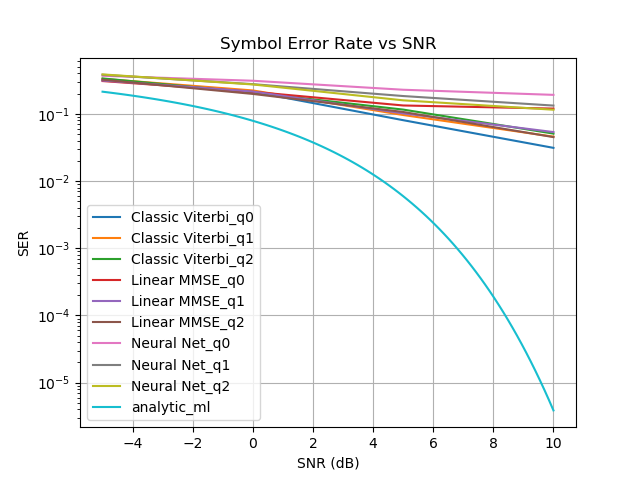
\includegraphics[width=\textwidth,height = 7cm]{results/quant_standard}


\item $p(y_{\mathrm{i}})$
: The probability of the channel being in a given state (including any randomness in the channel state) as well as the probability of the noise. This probability distribution function can be estimated using a mixture-model (Fig. \ref{fig:mm}) based on a set of received signal training data (In this case the same data used to train the neural network). In particular, the Expectation Maximization Algorithm is used with a chosen model for the channel. 
This term is constant over all states in a given step of the Viterbi algorithm and can therefore be interpretted as a term indicating the importance of the given time point on the total sequence path cost.
%picture of MM
%	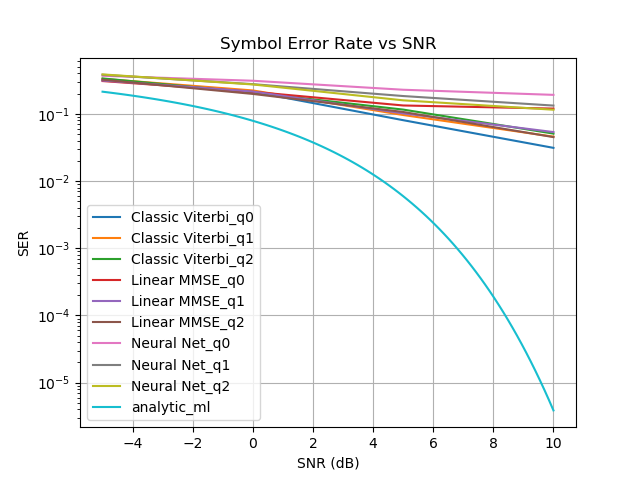
\includegraphics[width=\textwidth,height = 7cm]{results/quant_standard}
	\begin{figure}[H]
	\centering
	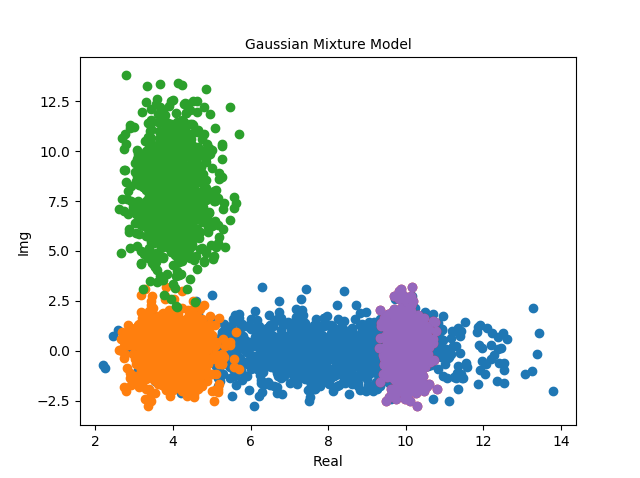
\includegraphics[width=10cm,height = 10cm]{system_model/mm}
	  \label{fig:mm}
	  	  \caption{Mixture Model }
	\end{figure}


\item $p(\mathbf{x}_{\mathrm{i-L+1}}^{\mathrm{i}})$
: The probability of a given transmitted sequence. This term can be neglected in the case of equiprobable symbols.

\end{itemize}

In summary, the metrics required by the Viterbi algorithm permit use of a neural network and mixture model to estimate the conditional probability distribution function $p(y_{\mathrm{i}}|\mathbf{x}_{\mathrm{i-L+1}}^{\mathrm{i}})$
\\

    \noindent\rule[16pt]{\textwidth}{0.6pt}
	Expectation Maximization Algorithm: (TODO Discuss how much derivation is needed here)

    \noindent\rule[10pt]{\textwidth}{0.4pt}
    {\footnotesize
    \begin{tabbing}
        {\bf given} $p(y_{\mathrm{i}}|x_{\mathrm{i-L+1}}^{\mathrm{i}}) \; \forall i \in {1..N}$ . \\*[\smallskipamount]
        {\bf for $i = 1..N $} \\
         \qquad \= {\bf for each state $s$ at time $i$}\\
        \qquad \qquad \= 1.\ Let $\textit{survivor cost}_{s}  += \text{min}\{\text{incoming transition costs}\}$ \\
%        \> 2.\ {\bf break if} $f(z) \leq \hat{f}_{\lambda}(z, x^{k})$. \\
%        \> 3.\ Update $\lambda := \beta \lambda$. \\*[\smallskipamount]
        {\bf return} Symbols corresponding to path of $\underset{s}{\text{argmin}} \; \textit{survivor cost}_{s} $
    \end{tabbing}}
    \noindent\rule[10pt]{\textwidth}{0.4pt}





\subsection{A Reduced State ViterbiNet}
While the Viterbi Algorithm complexity complexity scales exponentially in the number of states possible at each step of the algorithm, in some cases this complexity can be reduced without significant degradation of performance. In particular, if the system is such that some states are redundant, these can be combined. The following relevant example with state redundancy is posed and one potential method of reducing these states is considered. 

A received signal 
\begin{equation}
y[k] = \sum_{\mathrm{l=1}}^{\mathrm{L}} a[l]x[k-l] + n[k], \; n[k]  \sim \mathcal{N}(0,1)
\end{equation}

with $x[k-l] \in \{ -1, +1\}$ and $n[k]  \sim \mathcal{N}(0,1)$.  

In the case of a causal, LTI system with inter-symbol-interference $\mathbf{a} = [1, 0, .2, .2, .4]$ (with $\|\mathbf{a}\|^2_2 = 1$) the received signal (Fig.\ref{fig:redundant_channel}) has fewer than the potential $2^5$ states. As one of the channel taps is 0, this will have no impact and thus 16 of the potential 32 are removed. Further, as there are two taps with power 0.2 these can only represent 3 states. 

\begin{figure}[H]
\centering
	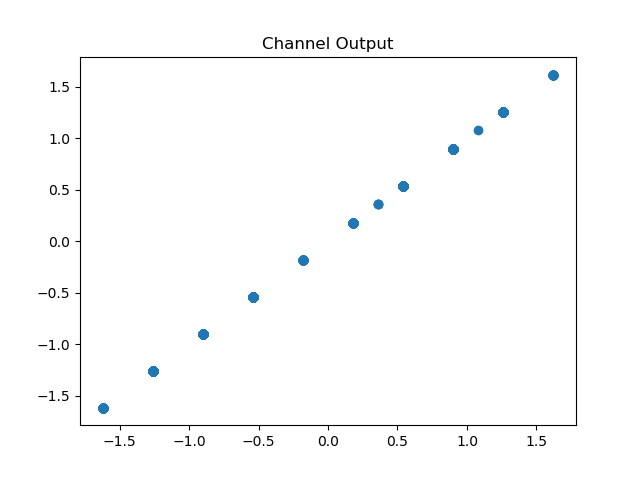
\includegraphics[width=10cm,height = 10cm]{system_model/channel_output}
	  \label{fig:redundant_channel}
	  	  \caption{LTI channel with state redundancy with high SNR}
\end{figure}

One way to exploit state redundancy is to cluster the original $2^L$ states into a set of $k$ clusters. The K-Means algorithm is proposed for clustering.
\\

    \noindent\rule[16pt]{\textwidth}{0.6pt}
K-Means Clustering: A method for unsupervised classification

    \noindent\rule[10pt]{\textwidth}{0.4pt}
    {\footnotesize
    \begin{tabbing}
        {\textbf{for} Number of Iterations}\\
         \qquad \= {\bf for each training point $x_{\mathrm{i}}, \;\mathrm{i}  \in \{1..N\}$}\\
        \qquad \qquad \= 1.\ Label $x_i$ with index of closest centroid using $\|x_{\mathrm{i}}- \text{closest}\|^2_2$ \\
        \qquad \= {\bf for centroid $L_{\mathrm{c}}, \;c \in \{1..C\}$}\\
                \qquad \qquad \= 1.\ Move $L_{\mathrm{c}}$ to average of all training points labeled "c"\\


%        \> 2.\ {\bf break if} $f(z) \leq \hat{f}_{\lambda}(z, x^{k})$. \\
%        \> 3.\ Update $\lambda := \beta \lambda$. \\*[\smallskipamount]
        {\bf return} Centroid locations
    \end{tabbing}}
    \noindent\rule[10pt]{\textwidth}{0.4pt}
    
Given a set of labeled training data, clustering reduces the number of channel states (and thus the Viterbi Algorithm Complexity) from $|\mathcal{A}|$ down to a number of clusters C. Choosing an appropriate number of clusters will influence the performance of the resulting decoder (Have figure showing this).
A implementation point to note is that after clustering the training data, the number of states must be increased by $|\mathcal{A}|$. The Viterbi algorithm selects a symbol sequence corresponding to a path of state transitions through the trellis. In order to make the correspondence between a unique path and a symbol sequence, each state transition must represent a transmitted symbol. \emph{Each} resulting centroid from the k-means clustering is associated to \emph{each} potential transmit symbol in order to create a "shorter" trellis for which each state transition still represents a transmitted symbol. 
Cite state reduction paper as motivation. 

Discuss minimum phase representations for channels and why this might be an advantage. 



\section{Simulation Results}
\subsection{System Model}
Consider the received signal 
\begin{equation}
y[k] = \sum_{\mathrm{l=1}}^{\mathrm{L}} a[l]x[k-l] + n[k], \; n[k]  \sim \mathcal{N}(0,1)
\end{equation}

with $x[k-l] \in \{ -1, +1\}$ and $n[k]  \sim \mathcal{N}(0,1)$.  
The resulting signal to noise ratio (SNR) is 
$\frac{E\{x[k]\}}{\sigma^2}$.

Unless noted, the neural network architecture and training are characterized by:
\begin{itemize}
\item Architecture: 4 layers {1, 100, 50, $M^L$}
\item Training Data Examples: 5000
\item Dropout Rate: .5
\item Neural Network Updates: Adam with step size $10^{-3}$ \cite{kingma2014adam}
\item Batch Size: 30 
\item Backpropogation Updates (Epochs): 300
\item Loss Function: Cross Entropy
\end{itemize}


\begin{figure}[H]
\centering
	  \caption{Simulation Channels: LTI Channel}
	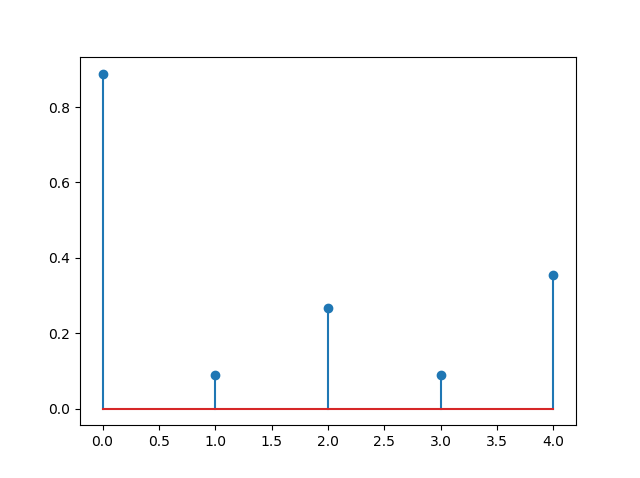
\includegraphics[width=10cm,height = 10cm]{system_model/lti_channel}
	  \label{fig:LTI Channel}
\end{figure}
\begin{figure}[H]
\centering
	  \caption{Simulation Channels: Quantizer}
	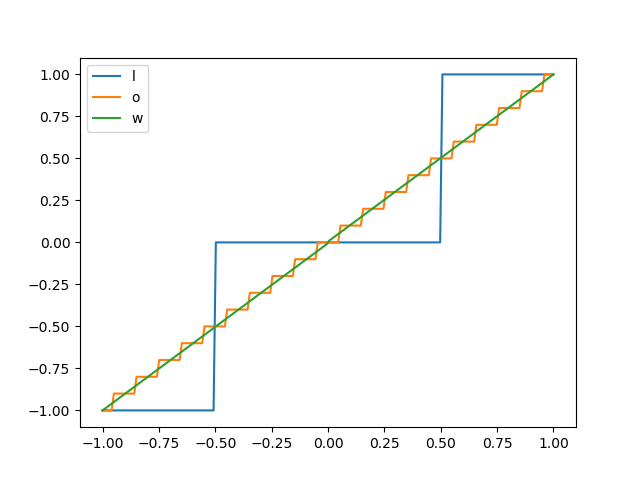
\includegraphics[width=10cm,height = 10cm]{system_model/quantizer}
	  \label{fig:Quantized Channel}
\end{figure}



Adding quantization at matched filter (prior to noise being added)


Details of NN architecture and training

Details of Mixture Model training


Consider the received signal 
\begin{equation}
y[k] = \sum_{\mathrm{l=1}}^{\mathrm{L}} a[l]x[k-l] + n[k], \; n[k]  \sim \mathcal{N}(0,1)
\end{equation}

with $x[k-l] \in \{ -1, +1\}$ and $n[k]  \sim \mathcal{N}(0,1)$.  
The resulting signal to noise ratio (SNR) is 
$\frac{E\{x[k]\}}{\sigma^2}$.


\begin{figure}[H]
\centering
	  \caption{Simulation Channels: LTI Channel}
	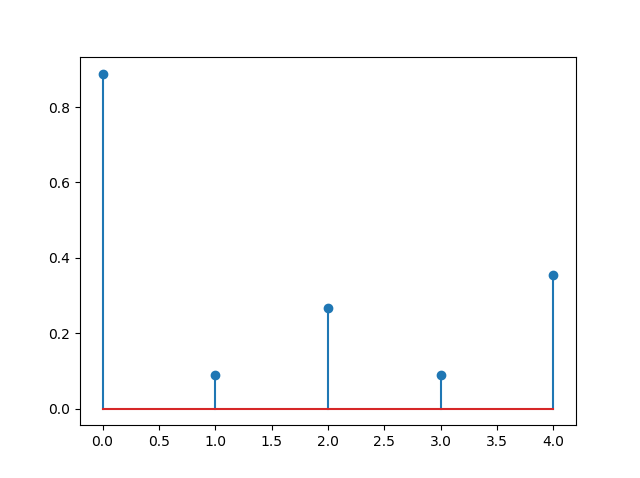
\includegraphics[width=10cm,height = 10cm]{system_model/lti_channel}
	  \label{fig:LTI Channel}
\end{figure}
\begin{figure}[H]
	  \caption{Simulation Channels: Quantizer}
	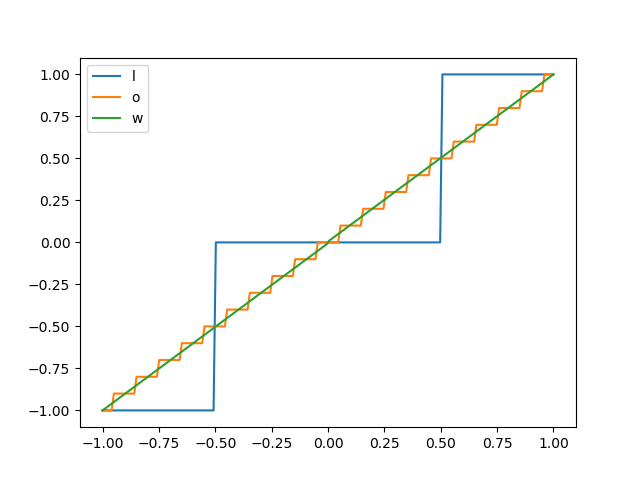
\includegraphics[width=10cm,height = 10cm]{system_model/quantizer}
	  \label{fig:Quantized Channel}
\end{figure}



Adding quantization at matched filter (prior to noise being added)


Details of NN architecture and training

Details of Mixture Model training

\subsection{Results}
proposed Figures
\begin{figure}[H]
	  \caption{LTI Channel performance}
	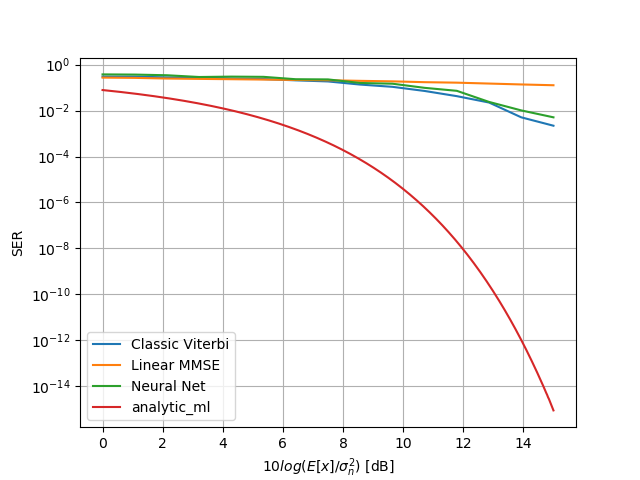
\includegraphics[width=\textwidth,height = 10cm]{results/lti_normal}
	  \label{fig:LTI Channel}
\end{figure}

\begin{figure}[H]
	  \caption{LTI + Quantized Channel performance}
	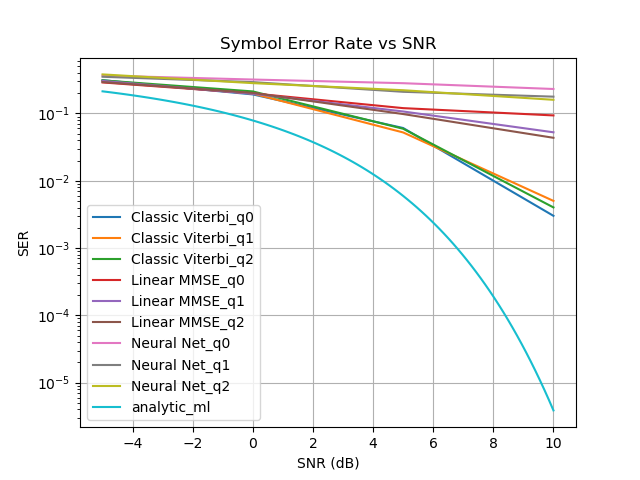
\includegraphics[width=\textwidth,height = 10cm]{results/lti_quantized}
	  \label{fig:LTI_quant Channel}
\end{figure}

\begin{figure}[H]
	  \caption{Reduced State ViterbiNet: LTI Channel}
	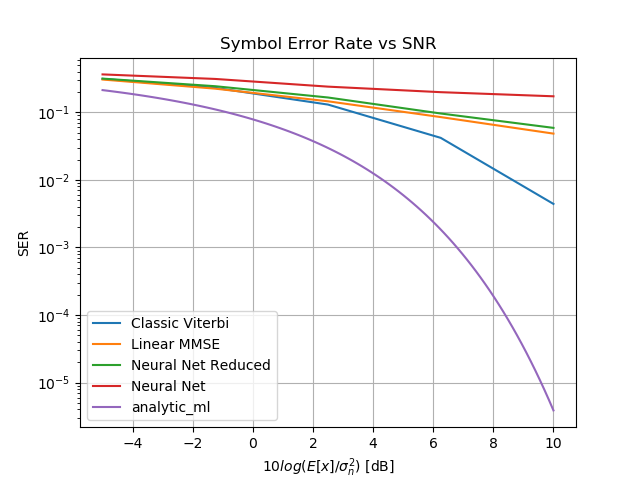
\includegraphics[width=\textwidth,height = 10cm]{results/lti_reduced}
	  \label{fig:reduced_lti}
\end{figure}

\begin{itemize}
\item ViterbiNet performance compared to MMSE and classic Viterbi LTI Channel

	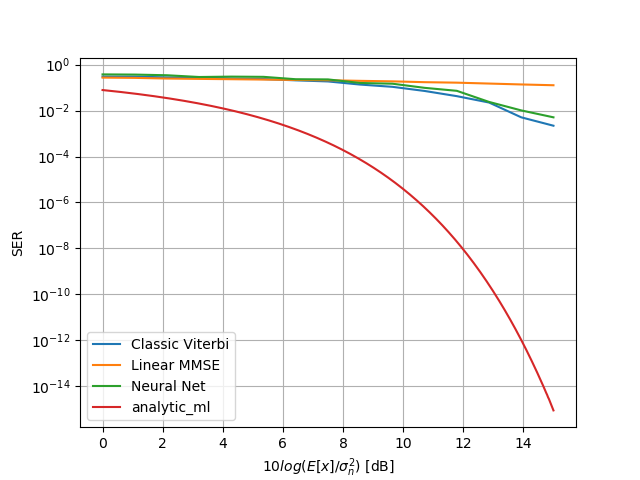
\includegraphics[width=\textwidth,height = 10cm]{results/lti_normal}

\item ViterbiNet performance compared to MMSE and classic Viterbi non-linear Channel

	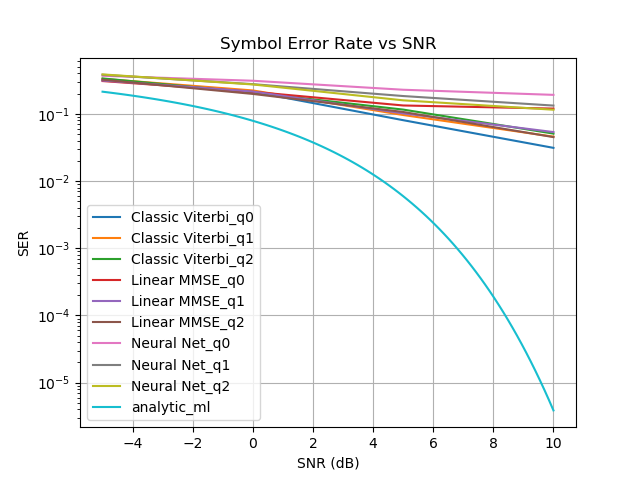
\includegraphics[width=\textwidth,height = 7cm]{results/quant_standard}

\item Reduced ViterbiNet on LTI Channel

	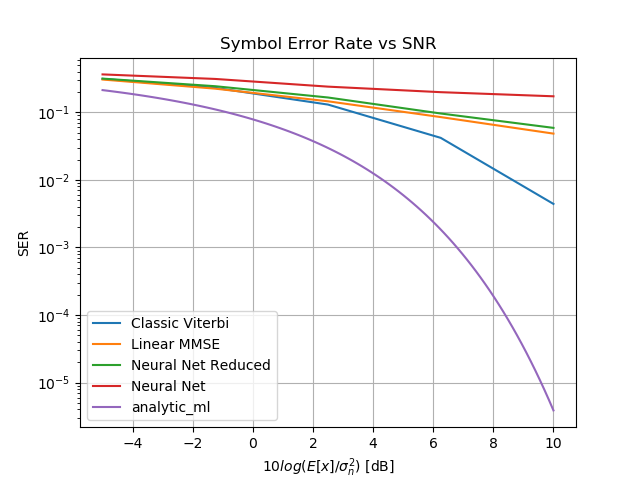
\includegraphics[width=\textwidth,height = 7cm]{results/lti_reduced}

\item Reduced ViterbiNet on non-linear Channel
%	\includegraphics[width=\textwidth,height = 7cm]{results/quant_reduced}

\end{itemize}
\subsection*{ViterbiNet}
\subsection*{Reduced State ViterbiNet}
\section{Conclusion}
\subsection{Future Work}
Discuss forward backward (App) algorithms that could be implemented.

\newpage
\bibliography{mc_report}
\end{document}
